%\documentclass[letterpaper, 10pt]{sigcomm-alternate}

\documentclass[peerreview, a4paper, 7pt]{IEEEtran}
%\documentclass[a4paper, 10pt]{IEEEtran}
%\documentclass{scrreprt}
\usepackage{times}
\usepackage{alltt}
\usepackage{graphicx}
\usepackage{alltt}
\usepackage{colortbl}
\usepackage[dvipsnames]{xcolor}

%\usepackage{color}
% \usepackage{caption2}
%\usepackage{subfigure}
%\usepackage{graphicx}
%\usepackage{colortbl}
%\usepackage[dvipsnames]{xcolor}
% \usepackage{ulem}

\usepackage{hyperref}

\pagenumbering{arabic}


%\ifx\pdfoutput\undefined
%\usepackage[pdfpagemode=none, pdfstartview=FitH, colorlinks=true, urlcolor=black, linkcolor=black, citecolor=black]{hyperref}
%\else
%\usepackage[pdftex, pdfpagemode=none, pdfstartview=FitH, colorlinks=true, urlcolor=black, linkcolor=black, citecolor=black, pdftex]{hyperref}
%\fi

\ifx\HCode\UnDef\else\hypersetup{tex4ht}\fi

%% Editorial work
% \newcommand{\purge}[1]{\textcolor{red}{\sout{#1}}}
% \newcommand{\add}[1]{\textcolor{blue}{#1}}

%%% End of editorial work.


 
\renewcommand{\em}[1]{\textit{#1}}
\begin{document}

\title{IPSO Smart Objects}

\author{\authorblockN{Jaime Jimenez\authorrefmark{1}, Michael Koster\authorrefmark{2}, Hannes Tschofenig\authorrefmark{3}\\}
\authorblockA{\authorrefmark{1}Ericsson, 
Email: jaime.jimenez@ericsson.com\\}
\authorblockA{\authorrefmark{2}SmartThings, 
Email: michael.koster@smartthings.com\\}
\authorblockA{\authorrefmark{3}ARM Limited, 
Email: hannes.tschofenig@arm.com\\}
\thanks{\textsc{Position paper for the 'IoT Semantic Interoperability Workshop 2016', 17$^{th}$ and 18$^{th}$ March 2016, San Jose, US.} The content of this document describes the current state of work at the IPSO Alliance. The document has been reviewed and approved by the IPSO Smart Object Committee.}
}

\date{\today}

\maketitle


\section{Introduction}

Standards for constrained devices are rapidly consolidating and the availability of IP on constrained devices enabled these devices to easily connect to the Internet. The IETF has also created a set of specifications for such IP-enabled devices to work in a Web-like fashion. One such protocol is the Constrained Application Protocol (CoAP)~\cite{rfc7252} that provides request/response methods, ways to identify resources, discovery mechanisms, etc. similar to HTTP~\cite{rfc2616} but for use in constrained environments.

On top of protocols like CoAP and HTTP there is a need for structuring data as well.

IPSO Smart Objects provide a common design pattern, an object model, to provide high level interoperability between Smart Object devices and connected software applications on other devices and services. IPSO Objects are defined in such a way that they do not depend on the use of CoAP, any RESTful protocol is sufficient. Nevertheless, to develop a complete and interoperable solution the Object model is based on the Open Mobile Alliance Lightweight Specification (OMA LWM2M)~\cite{lwm2m}, which is a set of management interfaces built on top of CoAP in order to enable device management operations (bootstrapping, firmware updates, error reporting, etc.). While LWM2M uses objects with fixed mandatory resources, IPSO Smart Objects use a more reusable design. 


\section{Data Model} 

The data model for IPSO Smart Objects consists of five parts:

\begin{enumerate}
\item Class Hierarchy
\item Schema
\item Data types 
\item Operations 
\item Content formats
\end{enumerate}

\subsection{Class Hierarchy}

The URI template follows standard Web Linking~\cite{rfc5988} and standard CoRE Link~\cite{rfc6690} formats. It defines an implicit class hierarchy consisting of Objects and Resources. The Object class is further split into ID and Instance subclasses. 

Objects are typed containers, which define the semantic type of instances. Instances inherit the type of their parent object, and allow Smart Object endpoints to expose multiple sensors and actuators of a particular type. Object instances are themselves containers for resources, which are the observable properties of an object. 

This class hierarchy allows application software to use simple APIs. For complex objects, linking of an object to another object through an object link resource is allowed. This enables the recursion to be handled at the object level, using design patterns similar to web linking. An application client can consume a device's API without knowing its structure and attributes a priori.

IPSO Smart Objects define the behavior at the object and resource level, for example the tracking of minimum and maximum values, resetting of accumulated values, etc.

\subsection{Schema}

The URI Template defined in LWM2M is used for IPSO Smart Objects consists of three unsigned 16-bit integers separated by the character '/' in the following form \textit{Object ID/Instance ID/Resource ID}

Semantically, the object type represents a single measurement, actuation, or control point, for example a temperature sensor, a light (actuator), or an on-off switch (control point).

The semantic meaning of a resource specifies a particular view or active property of an object. For example, a temperature sensor object might expose the current value (most recent reading), also the minimum and maximum possible reading, the minimum and maximum reading in an interval, and attributes like engineering units and application type.

Figure~\ref{temperature-uri-figure} shows an example URI of a temperature sensor. 

\begin{figure}[!t]
 \centering
 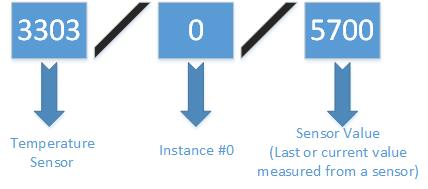
\includegraphics[scale=0.50]{temperature-uri.jpg}
 \caption{Temperature Sensor URI Example.}
 \label{temperature-uri-figure}
\end{figure}

Attributes describe the metadata configuration, settings, and state of an object or resource, and are discoverable by reading the link-format data of an object or resource. Multiple attributes may be serialized in the link-format descriptors that an object exposes. 

Some attributes are immutable for a given object or resource type. For example, the static read, write, and execute capability attributes are derived from a Smart Object's definition file, while other attributes, like the LWM2M Notification Attributes, are used to dynamically configure a particular object instance or resource.

Attributes are represented using the IETF CoRE Link-Format (RFC 6690) or an equivalent mapping to other content formats, for example, application/json+ld.

\subsection{Data Types}

IPSO Smart Objects re-use the data types defined in the OMA LWM2M specification~\cite{lwm2m}.

\begin{enumerate}
\item String: A UTF-8 string
\item Integer: An 8, 16, 32 or 64-bit signed integer.
\item Float: A 32 or 64-bit floating point value.
\item Boolean
\item Opaque: A sequence of binary octets.
\item Time: Unix Time.
\item Object Link: The object link is used to refer an instance of a given object. 
\end{enumerate}

\subsection{Operations}

IPSO Objects and their resources have the same operations as their counterparts in the OMA LWM2M specification~\cite{lwm2m} with the same semantics.

\begin{enumerate}
\item Resource values: Read, Write, Execute (restricted by the Access Type field)
\item Object Instances: Create, Delete (restricted by the Multiple Instances field)
\item Objects and their instances: Read, Write
\item Attributes: Set, Discover
\end{enumerate}

\subsection{Content Formats}

Content formats are those specified by the OMA LWM2M specification~\cite{lwm2m}:
\begin{enumerate}
\item Resource values: text/plain, tlv
\item Objects: text/senml+json, application/cbor, binary/tlv
\item Attributes: link-format, link-format+json
\end{enumerate}


\section{Composite Objects}

As devices increase in complexity (e.g., from a sensor to an appliance, from a switch to a complex actuator) the need to link resources to create more complex objects or "Composite Objects" arises. Such a composite object can, for example, be constructed with a single reusable type "generic composite object" with one ID. The resources may be of a generic reusable link type, also using a single ID, with multiple instances allowed. For example, '4000/0/6700/0' where 4000 is a "composite object" and 6700 is "generic object link". Composite objects offer higher granularity than one large nested object would. An observer of a device represented as a composite object could reduce bandwidth utilization by observing only the linked object instances instead of the full object. Figure~\ref{composite-object-figure} shows an example, performing a GET operation to the IPSO Thermostat Composite Object "/8300/0/7100" would retrieve an Object Link to "/3300/0".


\begin{figure}[!t]
 \centering
 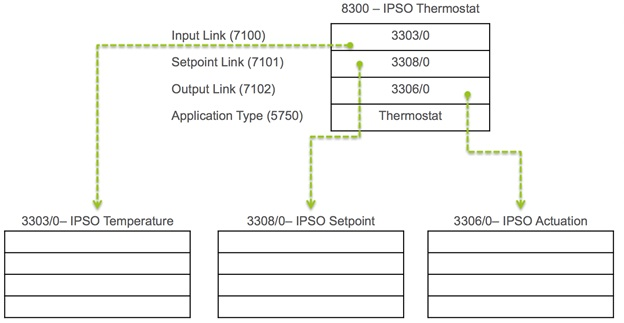
\includegraphics[scale=0.50]{composite-object.jpg}
 \caption{Composite Object Example.}
 \label{composite-object-figure}
\end{figure}

\section{Humidity Sensor Example}

Specification authors use different ways to describe resources exposed by IoT devices. Often natural text is used and sometimes more formal techniques are relied on. For the definition of the IPSO Smart Objects tables with natural language descriptions and XML (to offer machine-readable descriptions) are used.

The following is an example of a humidity sensor that contains the sensor value, units, min and max measured values, min and max range values and a resets for those. Figure~\ref{humidity-object-figure} shows the object and resource definitions in a tabular form and the definition in XML is shown in Appendix A. 

\begin{figure}[!t]
 \centering
 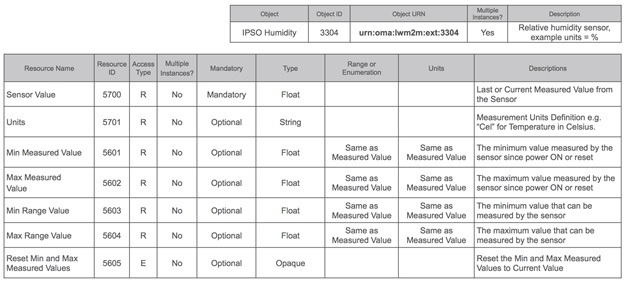
\includegraphics[scale=0.70]{humidity-object.jpg}
 \caption{IPSO Humidity Object Definition.}
 \label{humidity-object-figure}
\end{figure}

\section{IPSO Smart Objects}

\subsection{Starter Pack}

This IPSO Smart Objects Starter Pack describes 18 Smart Objects, including a temperature sensor, a light controller, an accelerometer, a presence sensor, and other types of sensors and actuators. These objects are common in many application domains. Appendix B shows the list of objects defined in the Starter Pack. 

With this initial publication the IPSO Alliance aimed to offer developers and standardization experts a starting point from which to build more complex objects in order to address vertical IoT market segments. One important design criteria in the design of the IPSO Smart Objects was and is to making it easy for developers to derive new objects based on their use case needs, while promoting interoperability to an extent as is practical. Naturally, a device that has not seen a newly defined object cannot know the semantics even if the contained resources can be understood on a syntactical level. However, re-use of existing object and resource definitions allows application developers to re-use code  

\subsection{Expansion Pack}

To complement the initial set of objects, the IPSO Smart Object Expansion Pack was published. The Expansion Pack adds 16 common template sensors, 6 special template sensors, 5 actuators and 6 control switch types.  

Some of the newly defined objects are generic in nature, such as voltage, altitude or percentage, while others are more specialized like the Color Object or the Gyrometer Object. New actuators and controllers are defined such as timer, buzzer, joystick and level. All of these objects were found to be necessary on a variety of use case domains.

Appendix C lists the objects defined in the IPSO Expansion Pack. 

\subsection{Extensibility}

Apart from the objects published by the IPSO Alliance developers and standardization experts are encouraged to define new objects tailored to their use cases if the already available functionality is insufficient. %IPSO offers a simple validation tool against the LWM2M schema, that developers can use [7]. 

The Starter and Expansion Pack provide basic examples for common sensors and actuators. Developers may extend the existing object set and submit them to IPSO. %with new ones and commit them to the "Application Specific Objects" repository of IPSO [8].

\bibliographystyle{IEEEtran}
% \bibliographystyle{acmtrans}
\bibliography{paper}


\appendix
\label{appendix_a}

\textsc{Appendix A: Humidity Object Definition in XML Format}

The following is the definition document for the Humidity Object in XML.

\begin{verbatim}
<?xml version="1.0" encoding="utf-8"?>
<LWM2M>
    <Object ObjectType="MODefinition">
        <Name>Humidity</Name>
        <Description1>This IPSO object should 
        be used with a humidity sensor to report a humidity 
        measurement.  It also provides resources for 
        minimum/maximum measured values and the minimum/maximum 
        range that can be measured by the humidity sensor. 
        An example measurement unit is relative humidity as a 
        percentage (ucum:%).
        </Description1>
        <ObjectID>3304</ObjectID>
        <ObjectURN>urn:oma:lwm2m:ext:3304</ObjectURN>
        <MultipleInstances>Multiple</MultipleInstances>
        <Mandatory>Optional</Mandatory>
        <Resources>
            <Item ID="5700">
                <Name>Sensor Value</Name>
                <Operations>R</Operations>
                <MultipleInstances>Single</MultipleInstances>
                <Mandatory>Mandatory</Mandatory>
                <Type>Float</Type>
                <RangeEnumeration></RangeEnumeration>
                <Units>Defined by "Units" resource.</Units>
                <Description>Last or Current Measured Value from 
                the Sensor
                </Description>
            </Item>
            <Item ID="5601">
                <Name>Min Measured Value</Name>
                <Operations>R</Operations>
                <MultipleInstances>Single</MultipleInstances>
                <Mandatory>Optional</Mandatory>
                <Type>Float</Type>
                <RangeEnumeration></RangeEnumeration>
                <Units>Defined by "Units" resource.</Units>
                <Description>The minimum value measured by the
                sensor since power ON or reset
                </Description>
            </Item>
            <Item ID="5602">
                <Name>Max Measured Value</Name>
                <Operations>R</Operations>
                <MultipleInstances>Single</MultipleInstances>
                <Mandatory>Optional</Mandatory>
                <Type>Float</Type>
                <RangeEnumeration></RangeEnumeration>
                <Units>Defined by "Units" resource.</Units>
                <Description>The maximum value measured by the 
                sensor since power ON or reset
                </Description>
            </Item>
            <Item ID="5603">
                <Name>Min Range Value</Name>
                <Operations>R</Operations>
                <MultipleInstances>Single</MultipleInstances>
                <Mandatory>Optional</Mandatory>
                <Type>String</Type>
                <RangeEnumeration></RangeEnumeration>
                <Units>Defined by "Units" resource.</Units>
                <Description>The minimum value that can be measured 
                by the sensor
                </Description>
            </Item>
            <Item ID="5604">
                <Name>Max Range Value</Name>
                <Operations>R</Operations>
                <MultipleInstances>Single</MultipleInstances>
                <Mandatory>Optional</Mandatory>
                <Type>Float</Type>
                <RangeEnumeration></RangeEnumeration>
                <Units>Defined by "Units" resource.</Units>
                <Description>The maximum value that can be measured 
                by the sensor
                </Description>
            </Item>
            <Item ID="5701">
                <Name>Sensor Units</Name>
                <Operations>R</Operations>
                <MultipleInstances>Single</MultipleInstances>
                <Mandatory>Optional</Mandatory>
                <Type>String</Type>
                <RangeEnumeration></RangeEnumeration>
                <Units></Units>
                <Description>Measurement Units Definition e.g. "Cel"
                for Temperature in Celsius.
                </Description>
            </Item>
            <Item ID="5605">
                <Name>Reset Min and Max Measured Values</Name>
                <Operations>E</Operations>
                <MultipleInstances>Single</MultipleInstances>
                <Mandatory>Optional</Mandatory>
                <Type>Opaque</Type>
                <RangeEnumeration></RangeEnumeration>
                <Units></Units>
                <Description>Reset the Min and Max Measured Values to
                Current Value
                </Description>
            </Item>
        </Resources>
        <Description2></Description2>
    </Object>
</LWM2M>\end{verbatim}

\textsc{Appendix B: IPSO Starter Pack}
\label{appendix_b}

The IPSO Starter Pack defines the objects shown in Table~\ref{ipso-start-pack-table}.

\begin{table}[!htbp]
\begin{center}
\caption{IPSO Starter Pack.}
\begin{tabular}{|l|c|}
\hline
\textbf{Object} & \textbf{Object ID}  \\
\hline\hline
Digital	& 3200 \\
\hline
Digital Output	& 3201\\
\hline
Analogue Input	& 3202\\
\hline
Analogue Output & 3203\\
\hline
Generic Sensor	& 3300\\
\hline
Illuminance Sensor & 3301\\
\hline
Presence Sensor	& 3302\\
\hline
Temperature Sensor & 3303\\
\hline
Humidity Sensor	& 3304\\
\hline
Power Measurement & 3305\\
\hline
Actuation & 3306\\
\hline
Set Point & 3308\\
\hline
Load Control & 3310\\
\hline
Light Control & 3311\\
\hline
Power Control & 3312\\
\hline
Accelerometer & 3313\\
\hline
Magnetometer & 3314\\
\hline
Barometer & 3315\\
\hline 
\end{tabular}
\label{ipso-start-pack-table}
\end{center}
\end{table}

\textsc{Appendix C: IPSO Expansion Pack }
\label{appendix_c}

The IPSO Expansion Pack defines the objects shown in Table~\ref{ipso-expansion-pack-table}.

\begin{table}[!htbp]
\begin{center}
\caption{IPSO Expansion Pack.}
\begin{tabular}{|l|c|}
\hline
\textbf{Object} & \textbf{Object ID}  \\
\hline\hline
Voltage	& 3316 \\
\hline
Current	& 3317 \\
\hline
Frequency & 3318 \\
\hline
Depth & 3319 \\
\hline
Percentage & 3320 \\
\hline
Altitude & 3321 \\
\hline
Load & 3322 \\
\hline
Pressure & 3323 \\
\hline
Loudness & 3324 \\
\hline
Concentration & 3325 \\
\hline
Acidity	 & 3326 \\
\hline
Conductivity & 3327 \\
\hline
Power & 3328 \\
\hline
Power Factor & 3329 \\
\hline
Rate & 3346 \\
\hline
Distance & 3330 \\
\hline
Energy & 3331 \\
\hline
Direction & 3332 \\
\hline
Time & 3333 \\
\hline
Gyrometer & 3334 \\
\hline
Color & 3335 \\
\hline
GPS Location & 3336 \\
\hline
Positioner & 3337 \\
\hline
Buzzer & 3338 \\
\hline
Audio Clip & 3339 \\
\hline
Timer & 3340 \\
\hline
Addressable Text Display & 3341 \\
\hline
On/Off Switch & 3342 \\
\hline
Push Button & 3347 \\
\hline
Level Control & 3343 \\
\hline
Up/Down Control & 3344 \\
\hline
Multistate Selector & 3348 \\
\hline
Multiple Axis Joystick & 3345 \\
\hline 
\end{tabular}
\label{ipso-expansion-pack-table}
\end{center}
\end{table}
\end{document}
